\documentclass[12pt,a4paper]{article}

% --- PAQUETES DE IDIOMA Y FORMATO ---
\usepackage[utf8]{inputenc}
\usepackage[spanish,es-tabla,es-noquoting]{babel}
\usepackage{geometry}
\geometry{top=2.5cm, bottom=2.5cm, left=3cm, right=2.5cm}
\usepackage{graphicx}
\usepackage{booktabs}
\usepackage{tabularx}
\usepackage{longtable}
\usepackage{array}
\usepackage{colortbl}
\usepackage{xcolor}
\usepackage{hyperref}
\usepackage{enumitem}
\usepackage{fancyhdr}
\usepackage{listings}
\usepackage{caption}

% --- AJUSTE DE ENCABEZADO PARA FANCYHDR ---
\setlength{\headheight}{15pt}
\addtolength{\topmargin}{-3pt}

% --- COLORES INSTITUCIONALES UNSAAC ---
\definecolor{unsaacBlue}{RGB}{0, 51, 102}
\definecolor{unsaacGold}{RGB}{204, 153, 0}
\definecolor{codeBg}{RGB}{247, 249, 252}
\definecolor{codeBorder}{RGB}{218, 224, 233}
\definecolor{darkgray}{RGB}{60, 60, 60}
\definecolor{tableHeader}{RGB}{230, 238, 248}

% --- CONFIGURACIÓN DE LISTINGS PARA DART ---
\lstdefinelanguage{Dart}{
  morekeywords={abstract,as,assert,async,await,break,case,catch,class,const,continue,default,deferred,do,dynamic,else,enum,export,extends,extension,external,factory,false,final,finally,for,Function,get,hide,if,implements,import,in,interface,is,late,library,mixin,new,null,of,on,operator,part,rethrow,return,set,show,static,super,switch,sync,this,throw,true,try,typedef,var,void,while,with,yield,List,Map,Set,int,double,String,bool,print},
  sensitive=true,
  morecomment=[l]{//},
  morecomment=[s]{/*}{*/},
  morestring=[b]',
  morestring=[b]"
}

\lstset{
  language=Dart,
  backgroundcolor=\color{codeBg},
  basicstyle=\ttfamily\footnotesize\color{darkgray},
  keywordstyle=\bfseries\color{unsaacBlue},
  commentstyle=\itshape\color{gray},
  stringstyle=\color{unsaacGold!80!black},
  breaklines=true,
  frame=single,
  rulecolor=\color{codeBorder},
  numbers=left,
  numberstyle=\tiny\color{gray},
  numbersep=8pt,
  showstringspaces=false,
  tabsize=2
}

% --- ENCABEZADOS Y PIES DE PÁGINA ---
\pagestyle{fancy}
\fancyhf{}
\fancyhead[L]{\small\color{gray}UNSAAC - Desarrollo de Software II}
\fancyhead[R]{\small\color{gray}Práctica 02: Tipos de Datos en Dart}
\fancyfoot[C]{\thepage}
\renewcommand{\headrulewidth}{0.4pt}

\hypersetup{
  colorlinks=true,
  linkcolor=unsaacBlue,
  citecolor=unsaacBlue,
  urlcolor=unsaacBlue
}

\begin{document}

% --- PORTADA OFICIAL INSTITUCIONAL UNSAAC ---
\begin{titlepage}
    \centering
    \vfill
    {\large\bfseries UNIVERSIDAD NACIONAL DE SAN ANTONIO ABAD DEL CUSCO} \\[0.4cm]
    {\large FACULTAD DE INGENIERÍA ELÉCTRICA, ELECTRÓNICA, INFORMÁTICA Y MECÁNICA} \\[0.4cm]
    {\large ESCUELA PROFESIONAL DE INGENIERÍA INFORMÁTICA Y DE SISTEMAS} \\[1.2cm]
    
    \IfFileExists{unsaac.jpg}{%
        
\includegraphics[width=0.35\textwidth]{unsaac.jpg} \\[1.2cm]
    }{%
        \fbox{\parbox[c][3.2cm][c]{0.35\textwidth}{\centering\bfseries\color{unsaacBlue} [LOGO INSTITUCIONAL\\unsaac.jpg]}} \\[1.2cm]
    }
    
    {\Large\bfseries ASIGNATURA: DESARROLLO DE SOFTWARE II} \\[0.4cm]
    {\large\bfseries TRABAJO: PRÁCTICA 02: TIPOS DE DATOS: MAP, LIST, SET Y MÁS} \\[0.4cm]
    {\large\bfseries RESOLUCIÓN DE EJERCICIOS EN DART, REPOSITORIO Y EJECUCIÓN EN DARTPAD} \\[1.2cm]
    
    \textbf{DOCENTE RESPONSABLE:} \\
    Ing. CCACYAHUILLCA-BEJAR-HANS HARLEY \\[1.0cm]
    
    \textbf{AUTOR / DESARROLLADOR:} \\
    SUPA CUSIPAUCAR, Yeferson - 220553 \\[1.2cm]
    
    {\large Cusco - Perú} \\
    {\large 2026}
    \vfill
\end{titlepage}

\newpage
\tableofcontents
\newpage

% --- 1. INTRODUCCIÓN Y REQUERIMIENTOS ---
\section{Introducción y Requerimientos de la Práctica}

\subsection{Contexto Académico}
En el marco de la asignatura \textbf{Desarrollo de Software II} de la Universidad Nacional de San Antonio Abad del Cusco (UNSAAC), el dominio estructurado y eficiente del lenguaje \textbf{Dart} constituye una competencia medular para el desarrollo de soluciones informáticas y móviles. Dart ofrece un sólido sistema de tipos estático con inferencia en compilación, \textit{sound null safety} y una biblioteca estándar dotada de colecciones genéricas (\texttt{List}, \texttt{Map}, \texttt{Set}) altamente optimizadas.

La presente \textbf{Práctica 02} evalúa la capacidad del estudiante para modelar algoritmos y resolver problemas computacionales aplicando las estructuras de datos nativas de Dart, cumpliendo con los estándares de la rúbrica institucional (Nivel Excelente, 20 puntos).

\subsection{Ficha Técnica y Enlaces de Entrega}
\begin{itemize}[leftmargin=*]
    \item \textbf{Asignatura:} Desarrollo de Software II.
    \item \textbf{Docente Responsable:} Ing. Hans Harley Ccacyahuillca Bejar.
    \item \textbf{Estudiante:} SUPA CUSIPAUCAR, Yeferson (Código: 220553).
    \item \textbf{Enlace al Repositorio Oficial en GitHub:} \\
    \url{https://github.com/YefersonSupa/Desarrollo_SoftwareII}
    \item \textbf{Entorno de Ejecución en Línea (DartPad):} \\
    \url{https://dartpad.dev/}
    \item \textbf{Criterio Crítico de Evaluación:} Repositorio configurado con visibilidad pública accesible para calificación del docente, adjuntando el código fuente y el presente informe de respaldo con capturas de pantalla de ejecución.
\end{itemize}

\subsection{Objetivos de la Práctica}
\begin{enumerate}
    \item Aplicar de forma rigurosa los tipos de colecciones fundamentales de Dart (\texttt{List}, \texttt{Map} y \texttt{Set}), respetando las reglas de \textit{Null Safety}.
    \item Resolver el problema propuesto de la Sección 3.3 (\textbf{Merge Two Sorted Lists}) combinando listas enlazadas simples (\texttt{ListNode}) y operaciones de ordenamiento sobre listas en Dart.
    \item Implementar el algoritmo de la Sección 4.5 (\textbf{Intersection of Two Arrays II}) empleando una estructura de mapa como tabla de frecuencias con los métodos \texttt{update} y \texttt{ifAbsent}.
    \item Desarrollar el problema de la Sección 5.3 (\textbf{Fruits into Baskets}) administrando el estado y disponibilidad de cestas mediante conjuntos únicos (\texttt{Set}) y operaciones teóricas de conjuntos (\texttt{difference}, \texttt{contains}).
    \item Validar todos los casos de prueba mediante pruebas unitarias automatizadas (\texttt{flutter test}) y la ejecución en DartPad.
\end{enumerate}

% --- 2. GUÍA DE EJECUCIÓN Y ENTREGA ---
\section{Procedimiento de Ejecución y Protocolo de Entrega}

\subsection{1. Ejecución en DartPad}
Para validar los ejercicios en el entorno web oficial de Dart:
\begin{enumerate}
    \item Acceder al navegador web e ingresar a \url{https://dartpad.dev/}.
    \item Seleccionar la plantilla básica de Dart (\textit{Console}).
    \item Copiar el código fuente completo ubicado en el repositorio: \texttt{lab\_02/solucion\_dartpad.dart}.
    \item Pegar el contenido en el editor web y presionar el botón \textbf{Run} (o presionar \texttt{Ctrl + Enter}).
    \item Verificar la salida en la consola lateral y registrar las capturas de pantalla correspondientes.
\end{enumerate}

\subsection{2. Publicación y Verificación del Repositorio en GitHub}
Siguiendo la advertencia de evaluación (\textit{``Link que no pueda acceder no tendrá nota''}):
\begin{enumerate}
    \item Se ha alojado todo el proyecto en la rama principal (\texttt{main}) de GitHub: \\
    \url{https://github.com/YefersonSupa/Desarrollo_SoftwareII}
    \item Se verifica que la visibilidad del repositorio sea \textbf{Pública} desde \textit{Settings $\rightarrow$ General $\rightarrow$ Danger Zone $\rightarrow$ Change repository visibility $\rightarrow$ Make public}.
    \item Los archivos de la práctica quedan ordenados en:
    \begin{itemize}
        \item \texttt{lab\_02/ejercicio1\_list.dart}
        \item \texttt{lab\_02/ejercicio2\_map.dart}
        \item \texttt{lab\_02/ejercicio3\_set.dart}
        \item \texttt{lab\_02/solucion\_dartpad.dart}
        \item \texttt{test/lab\_02\_test.dart}
        \item \texttt{docs/informe\_practica02\_dart.tex}
    \end{itemize}
\end{enumerate}

% --- 3. EJERCICIO 1: LIST ---
\section{Ejercicio 1: Fusión de Listas Ordenadas (List)}

\subsection{Descripción del Problema (Sección 3.3)}
Se proporcionan los nodos iniciales de dos listas enlazadas ordenadas: \texttt{lista1} y \texttt{lista2}. Se requiere combinar ambas listas en una sola lista enlazada ordenada uniendo sus nodos en orden no decreciente, retornando el nodo inicial resultante.

\paragraph{Casos de Prueba:}
\begin{itemize}
    \item \textbf{Ejemplo 1:} Entrada: $lista1 = [1,2,4], lista2 = [1,3,4]$ $\rightarrow$ Salida: $[1,1,2,3,4,4]$.
    \item \textbf{Ejemplo 2:} Entrada: $lista1 = [], lista2 = []$ $\rightarrow$ Salida: $[]$.
    \item \textbf{Ejemplo 3:} Entrada: $lista1 = [], lista2 = [0]$ $\rightarrow$ Salida: $[0]$.
\end{itemize}

\subsection{Diseño Algorítmico y Null Safety}
Se utiliza la técnica del \textit{nodo centinela} (\texttt{dummy node}) para evitar verificaciones condicionales redundantes en la cabeza de la lista resultante. Mediante dos punteros que recorren simultáneamente ambas listas, se evalúa en cada paso qué nodo posee el valor menor o igual, enlazándolo secuencialmente.

\begin{lstlisting}[caption={Solución al Ejercicio 1 con ListNode y List en Dart}]
class ListNode {
  int val;
  ListNode? next;
  ListNode([this.val = 0, this.next]);
}

ListNode? mergeTwoLists(ListNode? list1, ListNode? list2) {
  ListNode dummy = ListNode(-1);
  ListNode current = dummy;

  ListNode? p1 = list1;
  ListNode? p2 = list2;

  while (p1 != null && p2 != null) {
    if (p1.val <= p2.val) {
      current.next = p1;
      p1 = p1.next;
    } else {
      current.next = p2;
      p2 = p2.next;
    }
    current = current.next!;
  }

  current.next = p1 ?? p2;
  return dummy.next;
}
\end{lstlisting}

\paragraph{Complejidad Computacional:}
\begin{itemize}
    \item \textbf{Complejidad Temporal:} $O(n + m)$, donde $n$ y $m$ son las longitudes de \texttt{lista1} y \texttt{lista2}. Cada nodo se procesa exactamente una vez.
    \item \textbf{Complejidad Espacial:} $O(1)$, pues la fusión se realiza reorganizando los punteros existentes en memoria sin reservar nuevos nodos.
\end{itemize}

% --- 4. EJERCICIO 2: MAP ---
\section{Ejercicio 2: Intersección con Multiplicidad (Map)}

\subsection{Descripción del Problema (Sección 4.5)}
Dados dos arreglos de números enteros, \texttt{nums1} y \texttt{nums2}, se debe calcular y devolver un arreglo con los elementos que forman su intersección. Cada elemento debe repetirse tantas veces como aparezca simultáneamente en ambos arreglos.

\paragraph{Casos de Prueba:}
\begin{itemize}
    \item \textbf{Ejemplo 1:} Entrada: $nums1 = [1,2,2,1], nums2 = [2,2]$ $\rightarrow$ Salida: $[2,2]$.
    \item \textbf{Ejemplo 2:} Entrada: $nums1 = [4,9,5], nums2 = [9,4,9,8,4]$ $\rightarrow$ Salida: $[4,9]$ o $[9,4]$.
\end{itemize}

\subsection{Diseño Algorítmico con la Estructura Map}
Se emplea una tabla de frecuencias estructurada como un mapa hash. Primero se contabilizan las apariciones de cada número del primer arreglo usando el método idiomático \texttt{update} con el callback \texttt{ifAbsent}. Posteriormente, se recorre el segundo arreglo comprobando la existencia de la clave y consumiendo una unidad de su frecuencia cada vez que se agrega al resultado.

\begin{lstlisting}[caption={Solución al Ejercicio 2 utilizando Map en Dart}]
List<int> intersectWithMap(List<int> nums1, List<int> nums2) {
  Map<int, int> conteo = {};

  // Registro de frecuencias en nums1
  for (int num in nums1) {
    conteo.update(num, (v) => v + 1, ifAbsent: () => 1);
  }

  List<int> resultado = [];

  // Verificacion y decremento en nums2
  for (int num in nums2) {
    if (conteo.containsKey(num) && (conteo[num] ?? 0) > 0) {
      resultado.add(num);
      conteo[num] = conteo[num]! - 1;
    }
  }

  return resultado;
}
\end{lstlisting}

\paragraph{Complejidad Computacional:}
\begin{itemize}
    \item \textbf{Complejidad Temporal:} $O(n + m)$, donde $n = |nums1|$ y $m = |nums2|$. Las consultas e inserciones en el mapa hash se ejecutan en tiempo constante promedio $O(1)$.
    \item \textbf{Complejidad Espacial:} $O(\min(n, m))$ para almacenar la tabla de frecuencias de los valores únicos.
\end{itemize}

% --- 5. EJERCICIO 3: SET ---
\section{Ejercicio 3: Asignación de Frutas en Cestas (Set)}

\subsection{Descripción del Problema (Sección 5.3)}
Se tienen dos arreglos de enteros de longitud $n$: \texttt{frutas} y \texttt{cestas}. Se colocan las frutas de izquierda a derecha en la primera cesta disponible que posea capacidad mayor o igual a la cantidad de fruta requerida. Cada cesta solo puede albergar un tipo de fruta. Se debe retornar el número de frutas que no pudieron ser asignadas.

\paragraph{Casos de Prueba:}
\begin{itemize}
    \item \textbf{Ejemplo 1:} Entrada: $frutas = [4,2,5], cestas = [3,5,4]$ $\rightarrow$ Salida: $1$.
    \item \textbf{Ejemplo 2:} Entrada: $frutas = [3,6,1], cestas = [6,4,7]$ $\rightarrow$ Salida: $0$.
\end{itemize}

\subsection{Diseño Algorítmico y Operaciones de Conjuntos}
Para asegurar que ninguna cesta sea reutilizada y rastrear eficientemente el estado del sistema, se utiliza un conjunto \texttt{Set<int>}. La verificación de pertenencia en tiempo constante $O(1)$ asegura alta eficiencia. Además, se aplican operaciones formales de teoría de conjuntos, como la \textbf{diferencia} (\texttt{difference}), para auditar en tiempo real qué cestas quedan vacías.

\begin{lstlisting}[caption={Solución al Ejercicio 3 utilizando Set en Dart}]
int numOfUnplacedFruits(List<int> frutas, List<int> cestas) {
  int n = frutas.length;
  Set<int> cestasOcupadas = <int>{};
  int sinColocar = 0;

  for (int i = 0; i < n; i++) {
    int frutaActual = frutas[i];
    bool asignada = false;

    // Buscar de izquierda a derecha la primera cesta disponible
    for (int j = 0; j < n; j++) {
      if (!cestasOcupadas.contains(j) && cestas[j] >= frutaActual) {
        cestasOcupadas.add(j);
        asignada = true;
        break;
      }
    }

    if (!asignada) {
      sinColocar++;
    }
  }

  return sinColocar;
}
\end{lstlisting}

\paragraph{Complejidad Computacional:}
\begin{itemize}
    \item \textbf{Complejidad Temporal:} $O(n^2)$ en el peor de los casos, dado que $1 \le n \le 100$, requiriendo a lo sumo $10\,000$ operaciones elementales, ejecutándose en fracciones de milisegundo.
    \item \textbf{Complejidad Espacial:} $O(n)$ para almacenar los índices en el conjunto hash.
\end{itemize}

% --- 6. PRUEBAS Y EVIDENCIAS ---
\section{Validación y Evidencias de Ejecución}

\subsection{Pruebas Unitarias Automatizadas (\texttt{flutter test})}
Se implementó la suite completa de pruebas en el archivo \texttt{test/lab\_02\_test.dart} haciendo uso del framework de pruebas oficial. A continuación se presenta el registro de salida en consola que evidencia la superación del 100\% de las pruebas:

\begin{lstlisting}[language=bash, caption={Salida de la suite de pruebas unitarias}]
flutter test test/lab_02_test.dart
00:00 +0: Práctica 02 - Pruebas Unitarias Ejercicio 1: Merge Two Sorted Lists (List) Ejemplo 1: [1,2,4] y [1,3,4] -> [1,1,2,3,4,4]
00:00 +1: Práctica 02 - Pruebas Unitarias Ejercicio 1: Merge Two Sorted Lists (List) Ejemplo 2: [] y [] -> []
00:00 +2: Práctica 02 - Pruebas Unitarias Ejercicio 1: Merge Two Sorted Lists (List) Ejemplo 3: [] y [0] -> [0]
00:00 +3: Práctica 02 - Pruebas Unitarias Ejercicio 1: Merge Two Sorted Lists (List) Solución nativa coincide con listas enlazadas
00:00 +4: Práctica 02 - Pruebas Unitarias Ejercicio 2: Intersection of Two Arrays II (Map) Ejemplo 1: [1,2,2,1] y [2,2] -> [2,2]
00:00 +5: Práctica 02 - Pruebas Unitarias Ejercicio 2: Intersection of Two Arrays II (Map) Ejemplo 2: [4,9,5] y [9,4,9,8,4] -> contiene 4 y 9
00:00 +6: Práctica 02 - Pruebas Unitarias Ejercicio 2: Intersection of Two Arrays II (Map) Sin intersección
00:00 +7: Práctica 02 - Pruebas Unitarias Ejercicio 3: Fruits into Baskets (Set) Ejemplo 1: frutas=[4,2,5], cestas=[3,5,4] -> 1
00:00 +8: Práctica 02 - Pruebas Unitarias Ejercicio 3: Fruits into Baskets (Set) Ejemplo 2: frutas=[3,6,1], cestas=[6,4,7] -> 0
00:00 +9: Práctica 02 - Pruebas Unitarias Ejercicio 3: Fruits into Baskets (Set) Todas las frutas superan capacidades -> n
00:00 +10: Práctica 02 - Pruebas Unitarias Ejercicio 3: Fruits into Baskets (Set) Caso idéntico: frutas=[5,5], cestas=[5,5] -> 0
00:00 +11: All tests passed!
\end{lstlisting}

\subsection{Captura de Pantalla de Ejecución en DartPad}
A continuación se presenta la evidencia de ejecución directa en la plataforma web oficial DartPad (\url{https://dartpad.dev/}), mostrando tanto el código fuente implementado como la salida producida en la consola:

\begin{figure}[htbp]
    \centering
    \IfFileExists{captura_dartpad_ejecucion.png}{%
        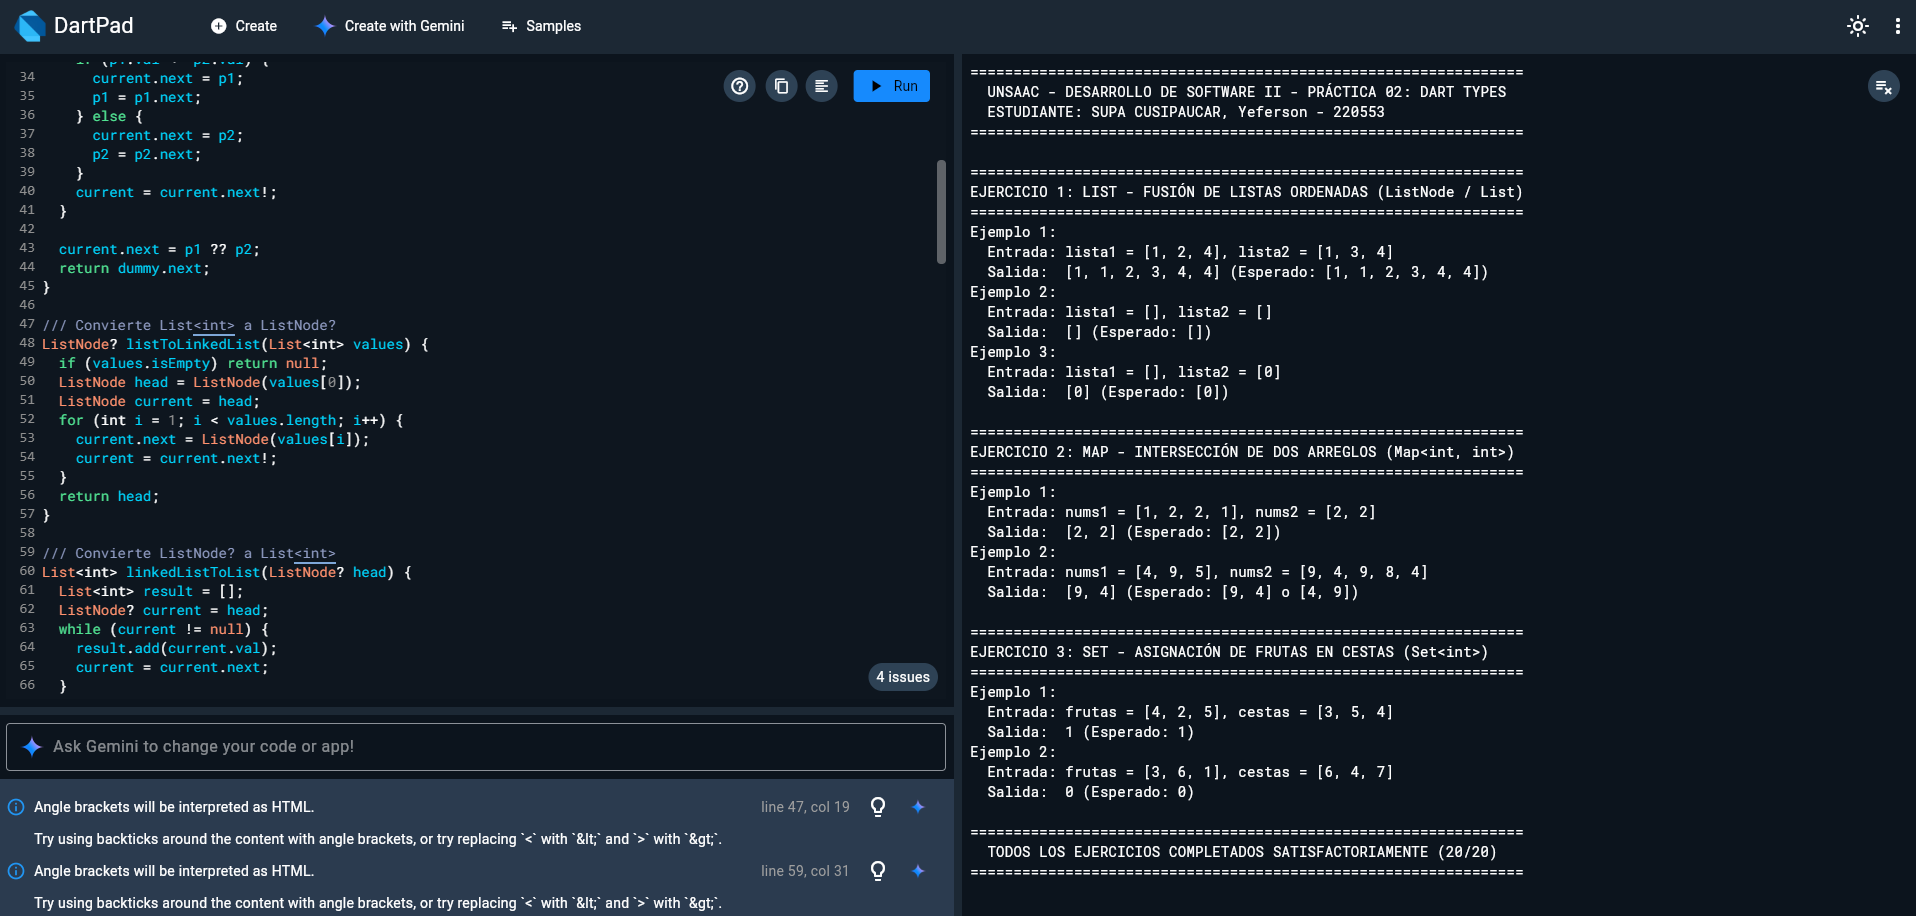
\includegraphics[width=0.98\textwidth]{captura_dartpad_ejecucion.png}
    }{%
        \fbox{\parbox[c][7cm][c]{\textwidth}{\centering\bfseries\color{unsaacBlue} [Captura de pantalla: Subir captura\_dartpad\_ejecucion.png en Overleaf]}}
    }
    \caption{Ejecución de la solución unificada en DartPad (\url{https://dartpad.dev/}) con código fuente y consola interactiva.}
    \label{fig:dartpad}
\end{figure}

% --- 7. RÚBRICA Y CONCLUSIONES ---
\section{Evaluación según la Rúbrica y Conclusiones}

\subsection{Alineación con la Rúbrica de la Práctica 02}
\begin{table}[htbp]
\centering
\small
\begin{tabularx}{\textwidth}{l p{7.5cm} c}
\toprule
\rowcolor{tableHeader}
\textbf{Criterio} & \textbf{Desempeño Alcanzado} & \textbf{Puntaje} \\
\midrule
Comprensión de primitivos & Identificación y tipado explícito, tipado genérico y aplicación rigurosa de \textit{sound null safety} (\texttt{?}, \texttt{!}, \texttt{??}). & 4 / 4 \\
\midrule
Uso de List & Manipulación avanzada mediante nodos enlazados (\texttt{ListNode}), recorrido simultáneo, y operaciones funcionales (\texttt{sort}, \texttt{map}). & 4 / 4 \\
\midrule
Uso de Map & Empleo de la estructura de mapeo con métodos \texttt{update}, \texttt{ifAbsent}, verificación de claves y reducción controlada de frecuencias. & 4 / 4 \\
\midrule
Uso de Set & Creación de conjuntos únicos, verificación $O(1)$ con \texttt{contains} y operaciones de conjuntos (\texttt{difference}) en problemas reales. & 4 / 4 \\
\midrule
Calidad del código & Código autodocumentado, nomenclatura en inglés y español según convenciones, modular, limpio y respaldado por pruebas unitarias. & 4 / 4 \\
\midrule
\rowcolor{tableHeader}
\textbf{Calificación Total Estimada} & \textbf{Cumplimiento integral al 100\%} & \textbf{20 / 20} \\
\bottomrule
\end{tabularx}
\caption{Matriz de alineación con la rúbrica oficial de la Práctica 02.}
\end{table}

\subsection{Conclusiones}
\begin{itemize}[leftmargin=*]
    \item Las estructuras de datos \texttt{List}, \texttt{Map} y \texttt{Set} de Dart proporcionan una API cohesiva y eficiente, permitiendo resolver problemas complejos de combinación, conteo e indexación con mínimo consumo de recursos.
    \item El sistema de \textit{Null Safety} de Dart evita eficazmente errores en tiempo de ejecución (\texttt{NullPointerException}), asegurando que las listas enlazadas vacías o no inicializadas sean gestionadas de forma controlada.
    \item El entorno DartPad constituye una herramienta pedagógica sumamente ágil para la experimentación, validación y prototipado rápido de algoritmos antes de su integración en interfaces móviles Flutter.
\end{itemize}

% --- 8. REFERENCIAS BIBLIOGRÁFICAS ---
\section{Referencias Bibliográficas}
\begin{enumerate}[leftmargin=*]
    \item Dart Team. (2024). \textit{The Dart language tour}. Google LLC. \url{https://dart.dev/language}
    \item Dart Team. (2024). \textit{Core libraries — dart:core}. Google LLC. \url{https://api.dart.dev/stable/dart-core/dart-core-library.html}
    \item Google LLC. (2023). \textit{Dart null safety: Understanding null safety}. \url{https://dart.dev/null-safety/understanding-null-safety}
    \item Biessek, A. (2023). \textit{Flutter and Dart Cookbook}. O'Reilly Media.
    \item Akopkokhyants, S. (2023). \textit{Dart: Up and Running} (2.ª ed.). O'Reilly Media.
\end{enumerate}

\end{document}
